%	$Id: minerror.tex,v 1.4 1998/08/19 11:48:33 goossens Exp goossens $	
%%%%%%%%%%%%%%%%%%%%%%%%%%%%%%%%%%%%%%%%%%%%%%%%%%%%%%%%%%%%%%%%%%%
%                                                                 %
%   MINUIT User Guide -- LaTeX Source                             %
%                                                                 %
%   Part 2: Chapter on error interpretation                       %
%                                                                 %
%   The following external EPS files are referenced:              %
%      minoserr.eps,minosco1.eps,minosco2.eps,minosco3.eps        %
%                                                                 %
%   Editor: Michel Goossens / CN-AS                               %
%   Last Mod.: 26 Jan. 1993 18:00 mg                              %
%                                                                 %
%%%%%%%%%%%%%%%%%%%%%%%%%%%%%%%%%%%%%%%%%%%%%%%%%%%%%%%%%%%%%%%%%%%
 
\chapter{Interpretation of the errors on Minuit parameters}
 
It often happens that the solution of a minimization problem using
Minuit is itself straightforward, but the calculation or
interpretation of the resulting parameter uncertainties is
considerably more complicated. The purpose of this chapter is to
clarify the most commonly encountered difficulties in parameter error
determination. These difficulties may arise in connection with any
fitting program, are discussed here with Minuit terminology.
 
The most common causes of misinterpretation may be grouped into 
three categories:
 
\begin{OL}
\item Proper normalization of the user-supplied chi-square or
  likelihood function, and appropriate \Cind[SET ERRordef]{ERROR DEF}.
\item Non-linearities in the problem formulation, leading to different
  errors being calculated by different techniques, such as
  \Cind[MIGrad]{MIGRAD}, \Cind[HESse]{HESSE} and \Cind[MINos]{MINOS}.
\item Multiparameter error definition and interpretation.
\end{OL}
 
All these topics are discussed in some detail in Eadie et
al.\cite{bib-EADIE}, which may be consulted for further details.
 
\section{Function normalization and ERROR DEF}
 
In order to provide for full generality in the user-defined function
value, the user is allowed to define a normalization factor known
internally as \texttt{UP} and defined by the Minuit user on an
\Cind[SET ERRordef]{ERROR DEF} command card.  The default value is
one. The Minuit error on a parameter is defined as the change of
parameter which would produce a change of the function value equal to
\texttt{UP}.  This is the most general way to define the error,
although in statistics it is more usual to define it in terms of the
second derivative of the $\chi^2$ function -- with respect to the
parameter in question. In the simplest linear case (when the function
is exactly parabolic at the minimum), the value \texttt{UP=1.0}
corresponds to defining the error as the inverse of the second
derivative at the minimum. The fact that Minuit defines the error in
terms of a function change does not mean that it always calculates
such a function change. Indeed it sometimes (\Cind[HESse]{HESSE})
calculates the second derivative matrix and inverts it, assuming a
parabolic behaviour. This distinction is discussed in section
\ref{sec:errornonlin}.
 
The purpose of defining errors by function changes is threefold: 

\begin{OL}
\item to preserve its meaning in the non-parabolic case (see section
  \ref{sec:errornonlin});
\item to allow generality when the user-defined function is not a chi-
  square or likelihood, but has some other origin;
\item to allow calculation not only of ``one-standard deviation''
  errors, but also two or more standard deviations, or more general
  'confidence regions', especially in the multiparameter case (see
  section \ref{sec:errormultipar}).
\end{OL}
 
\subsection{Chi-square normalization}
 
If the user's function value $F$ is supposed to be a chisquare, it must 
of course be properly normalized. That is, the ``weights'' must in fact 
correspond to the one-standard-deviation errors on the observations. 
The most general expression for the chi-square $\chi$ is of 
the form (see \cite{bib-EADIE}, p.163):
 
\[ \chi^2 = \sum_{i,j} (x_i - y_i(a)) V_{ij} (x_j - y_j(a)) \]
 
where $x$ is the vector of observations, $y(a)$ is the vector of fitted 
values (or theoretical expressions for them) containing the variable 
fit parameters $a$, and $V$ is the inverse of the error matrix of the 
\index{covariance matrix}
observations $x$, also known as the covariance matrix of the 
observations.
 
Fortunately, in most real cases the observations $x$ are statistically 
independent of each other (e.g., the contents of the bins of a 
histogram, or measurements of points on a trajectory), so the 
matrix $V$ is diagonal only. The expression for $\chi^2$ then simplifies to 
the more familiar form:
 
\[ \chi^2 = \sum_{i} \frac{(x_i - y_i(a))^2}{e_i^2} \]
 
where $e^2$ is the inverse of the diagonal element of $V$, the square of 
the error on the corresponding observation $x$. In the case where the $x$
are integer numbers of events in an unweighted histogram, for 
example, the $e^2$ are just equal to the x (or to the y, see \cite{bib-EADIE},
pp.170-171).
 
The minimization of $\chi^2$ above is sometimes called {\bf weighted least 
\index{weighted least squares}%
\index{least squares!weighted}%
squares} in which case the inverse quantities $1/e^2$ are called the weights. 
Clearly this is simply a different word for the same thing, 
but in practice the use of these words sometimes means that the 
interpretation of $e^2$ as variances or squared errors is not 
straightforward. The word weight often implies that only the 
relative weights are known (``point two is twice as important as 
point one'') in which case there is apparently an unknown overall 
normalization factor. Unfortunately the parameter errors coming out 
of such a fit will be proportional to this factor, and the user must be 
aware of this in the formulation of his problem.
                                                                                               
The $e^2$ may also be functions of the fit parameters $a$ (see \cite{bib-EADIE},
pp.170-171). Normally this results in somewhat slower convergence 
of the fit since it usually increases the nonlinearity of the fit. (In 
the simplest case it turns a linear problem into a non-linear one.) 
However, the effect on the fitted parameter values and errors should 
be small.
 
If the user's chi-square function is correctly normalized, he should 
\index{standard deviation}
use \texttt{UP=1.0} (the default value) to get the usual 
one standard-deviation errors for the parameters one by one. 
To get two-standard-dev.eviation
errors, use \Cind[SET ERRordef]{ERROR DEF 4.0}, etc., 
since the chisquare dependance on 
parameters is quadratic. For more general confidence regions 
involving more than one parameter, see section \ref{sec:errornonlin}.
 
\subsection{Likelihood normalization}
\index{likelyhood}

If the user function is a negative log-likelihood function, it must 
again be correctly normalized, but the reasons and ensuing problems 
in this case are quite different from the chisquare case. The 
likelihood function takes the form (see \cite{bib-EADIE}, p. 155):
 
\[ F = - \sum_{i} \ln f(x_i,a) \]
 
where each $x$ represents in general a vector of observations, the $a$ 
are the free parameters of the fit, and the function $f$ represents the 
hypothesis to be fitted. This function $f$ must be normalized:
 
\[ \int f(x_i,a) \mathrm{d}x_1 \mathrm{d}x_2 \ldots 
                 \mathrm{d}x_n = \mathrm{constant} \]
 
that is, the integral of $f$ over all observation space $x$ must be 
independent of the fit parameters $a$.
 
The consequence of not normalizing $f$ properly is usually that the fit 
simply will not converge, some parameters running away to infinity. 
Strangely enough, the value of the normalization constant does not 
affect the fitted parameter values or errors, as can be seen by the 
fact that the logarithm makes a multiplicative constant into an 
additive one, which simply shifts the whole log-likelihood curve and 
affects its value, but not the fitted parameter values or errors. In 
fact, the actual value of the likelihood at the minimum is quite 
meaningless (unlike the chi-square value) and even depends on the 
units in which the observation space $x$ is expressed. The meaningful 
quantity is the difference in log-likelihood between two points in 
parameter-space, which is dimensionless.
 
For likelihood fits, the value \texttt{UP=0.5} corresponds to 
one-standard-deviation errors. 
Or, alternatively, $F$ may be defined as $-2\log(\mathrm{likelihood})$, 
in which case differences in $F$ have the same meaning as for chi-square 
and \texttt{UP=1.0} is appropriate. The two different ways of introducing the 
factor of 2 are quite equivalent in Minuit, and although most people 
seem to use \texttt{UP=0.5}, it is perhaps more logical to put the 
factor 2 directly into \Rind{FCN}.
 
\section{Non-linearities: MIGRAD versus HESSE versus MINOS}
\label{sec:errornonlin}

In the theory of statistics, one can show that in the asymptotic
limit, any of several methods of determining parameter errors are
equivalent and will give the same result.  Let us for the moment call
these methods \Cind[MIGrad]{MIGRAD}, \Cind[HESse]{HESSE}, and
\Cind[MINos]{MINOS} (\Cind[SIMplex]{SIMPLEX} is a special case).  It
turns out that the conditlons under which these methods yield exactly
the same errors are either of the following:
 
\begin{OL}
\item The model to be fitted ($y$ or $f$) is exactly a linear function of the 
      fit parameters $a$, or
\item The amount of observed data is infinite.
\end{OL}
 
It may happen that (1) is  satisfied, in whlch case you don't really 
need Minuit, a smaller, simpler, and faster program would do, since 
a linear problem can be solved directly without iterations (see \cite{bib-EADIE},
p. 163-165), for example with CERN library program \texttt{LSQQR}. 
Nevertheless, it may be convenient to use Minuit slnce non-linear 
terms can then be added later if desired, without major changes to 
the method. Condition (2) is of course never satisfied, although in 
practice it often happens that there is enough data to make the 
problem ``almost linear'', that is there is so much data that the 
range of parameters allowed by the data becomes very small, and 
any physical function behaves linearly over a small enough region.
 
The following sections explain the dirrerences between the various 
parameter errors given by Minuit.
 
\subsection{Errors printed by Minuit}
 
The errors printed by Minuit at any given stage represent the best 
symmetric error estimates available at that stage, which may not 
be very good. For example, at the first entry to \Rind{FCN}, the user's step 
slzes are given, and these may bear no resemblance at all to proper 
parameter errors, although they are supposed to be order-of-magnltude estimates. 
After crude minimizers like \Cind[SEEk]{SEEK} or \Cind[SIMplex]{SIMPLEX}, 
a revised error estimate may be given, but this too is only meant to
be an order-or-magnitude estimate, and must certainly not be 
taken seriously as a physical result. Such numbers are mainly for 
the internal use of Minuit, which must after all assume a step size 
for future minimizations and derivative calculations, and uses these 
``errors'' as a first guess to be modified on the basis of experience.
 
\subsection{Errors after MIGRAD (or MINIMIZE)}
 
The minimizing technique currently implemented in \Cind[MIGrad]{MIGRAD} is a 
stable variation (the ``switching'' method) of the 
Davidon-Fletcher-Powell variable-metric algorithm.
This algorithm converges to the correct error matrix as it converges 
to the function minimum. 

This algorithm requires at each step a ``working approximation'' of the
error matrix, and a rather good approximation to the gradient vector at
the current best point. 
The starting approximation to the error matrix may be obtained in different
ways, depending on the status of the error matrix before MIGRAD is called
as well as the value of STRATEGY.  Usually it is found to be advantageous 
to evaluate the error matrix rather carefully at the start point in order
to avoid premature convergence, but in principle even the unit matrix
can be used as a starting approximation.  
Usually the Minuit default is to start by calculating the full error matrix by
calculating all the second derivatives and inverting the matrix.
If the user wants to make sure this is done, he can call HESSE before MIGRAD.

If a unit matrix is taken to start,
then the first step will be in a {\em steepest descent} direction, which is
not bad, but the estimate of EDM, needed to judge convergence, will be poor.
At each successive step, the information gathered from the change of gradient
is used to improve the approximation to the error matrix, without the need
to calculate any second derivatives or invert any matrices.
The algorithm used for this {\em updating} is supposed to be the best known,
but if there are a lot of highly correlated parameters, it may take many steps
before the off-diagonal elements of the error matrix approach the correct values.

In practice, \Cind[MIGrad]{MIGRAD} usually yields good estimates of the 
error matrix, but it is not absolutely reliable for two reasons:
 
\begin{OL}
\item Convergence to the minimum may occur ``too fast'' for \Cind[MIGrad]{MIGRAD} to 
      have a good estimate of the error matrix. In the most flagrant of 
      such cases, \Cind[MIGrad]{MIGRAD} realizes this and automatically introduces an 
      additional call to \Cind[HESse]{HESSE} (described below), informing the user that 
      the covariance matrix is being recalculated. Since, for $n$ variable 
      parameters, there are $n(n+1)/2$ elements in the error matrix, the 
      number of \Rind{FCN} calls from \Cind[MIGrad]{MIGRAD} must be large compared with 
      $n^2$ in order for the \Cind[MIGrad]{MIGRAD} error matrix calculation to be 
      reliable.
\item \Cind[MIGrad]{MIGRAD} gathers information about the error matrix as it 
      proceeds, based on function values calculated away from the 
      minimum and assuming that the error matrix is nearly constant as a 
      function of the parameters, as it would be if the problem were 
      nearly linear. If the problem is highly non-linear, the error matrix 
      will depend strongly on the parameters, \Cind[MIGrad]{MIGRAD} will converge more 
      slowly, and the resulting error matrix will at best represent some 
      average over the last part of the trajectory in parameter-space 
      traversed by \Cind[MIGrad]{MIGRAD}.
\end{OL}
 
If \Cind[MIGrad]{MIGRAD} errors are wrong because of (1),
\Cind[HESse]{HESSE} should be commanded after \Cind[MIGrad]{MIGRAD} 
and will give the correct errors. If \Cind[MIGrad]{MIGRAD} 
errors are wrong because of (2), \Cind[HESse]{HESSE} will help, but only in an 
academic sense, since in this case the error matrix is not the whole 
story and for proper error calculation \Cind[MINos]{MINOS} must be used.
 
As a general rule, anyone seriously interested in the parameter 
errors should always put at least a \Cind[HESse]{HESSE} command after each 
\Cind[MIGrad]{MIGRAD} (or \Cind[MINImize]{MINIMIZE}) command.
 
\subsection{Errors after HESSE}
 
\Cind[HESse]{HESSE} simply calculates the full second-derivative matrix by finite 
differences and inverts it. It therefore calculates the error matrix 
at the point where it happens to be when it is called. If the error 
matrix is not positive-definite, diagnostics are printed, and an 
\index{error matrix}
attempt is made to form a positive-definite approximation. The 
error matrix must be positive-definite at the solution (minimum) 
for any real physical problem. It may well not be positive away from 
the minimum, but most algorithms including the \Cind[MIGrad]{MIGRAD} algorithm 
require a positive-definite ``working matrix''.
 
The error matrix produced by \Cind[HESse]{HESSE} is used to calculate what Minuit 
prints as the parameter errors, which therefore contain the effects 
due to parameter correlations. The extent of the two-by-two 
correlations can be seen from the correlation coefficients printed by 
Minuit, and the global correlations (see \cite{bib-EADIE}, p. 23) are also 
printed. All of these correlation coefficients must be less than one 
in absolute value. If any of them are very close to one or minus one, 
this indicates an illposed problem with more free parameters than 
can be determined by the model and the data.
 
\subsection{Errors by MINOS}
 
\Cind[MINos]{MINOS} is designed to calculate the correct errors in all cases, 
especially when there are non-linearities as described above. The 
theory behind the method is described in \cite{bib-EADIE}, pp. 204-205 
(where ``non-parabolic likelihood'' should of course read 
``non-parabolic log-likelihood'', 
which is equivalent to ``nonparabolic chi-square'').
 
\Cind[MINos]{MINOS} actually follows the function out from the minimum to find 
where it crosses the function value (minimum + \texttt{UP}), instead of using 
the curvature at the minimum and assuming a parabolic shape. This 
method not only yields errors which may be different from those of 
\Cind[HESse]{HESSE}, but in general also different positive and negative errors 
(asymmetric error interval). Indeed the most frequent result for 
most physical problems is that the (symmetric) \Cind[HESse]{HESSE} error lies 
between the positive and negative errors of \Cind[MINos]{MINOS}. The difference 
between these three numbers is one measure of the non-linearity of 
the problem (or rather of its formulation).
 
In practice, \Cind[MINos]{MINOS} errors usually turn out to be close to, or 
somewhat larger than errors derived from the error matrix, although 
in cases of very bad behaviour (very little data or ill-posed model) 
anything can happen. In particular, it is often not
true in \Cind[MINos]{MINOS} that two-standard-deviation errors 
(\texttt{UP=4}) and three-standard-deviation  errors (\texttt{UP=9}) 
are respectively two and three times as big as one-standard-deviation errors, 
as is true by definition for errors derived from the 
error matrix (\Cind[MIGrad]{MIGRAD} or \Cind[HESse]{HESSE}).

\section{Multiparameter errors}
\label{sec:errormultipar}
 
In addition to the difficulties described above, a special class of 
problems arise in interpreting errors when there is more than one 
free parameter. These problems are quite separate from those 
described above and are really much simpler in principle, although in 
practice confusion often arises.
 
\subsection{The Error Matrix}
\index{error matrix}
\index{covariance matrix}
 
The error matrix, also called the covariance matrix, is the inverse of 
the second derivative matrix of the (log-likelihood or chisquare) 
function with respect to its free parameters, usually assumed to be 
evaluated at the best parameter values (the function minimum). The 
diagonal elements of the error matrix are the squares of the 
\index{correlations}%
individual parameter errors, {\bf including the effects of correlations}
with the other parameters.
 
The inverse of the error matrix, the second derivative matrix, has as 
diagonal elements the second partial derivatives with respect to one 
parameter at a time. These diagonal elements are not therefore 
coupled to any other parameters, but when the matrix is inverted, 
the diagonal elements of the inverse contain contributions from all 
the elements of the second derivative matrix, which is ``where the 
correlations come from''.
 
Although a parameter may be either positively or negatively 
correlated with another, the effect of correlations is always to 
increase the errors on the other parameters in the sense that if a 
given free parameter suddenly became exactly known (fixed), that 
would always decrease (or at least not change) the errors on the 
other parameters. In order to see this effect quantitatively, the 
following procedure can be used to ``delete'' one parameter from the 
error matrix, including its effects on the other parameters:
 
\begin{OL}
\item Invert the error matrix, to yield the second-derivative matrix.
\item Remove the row and column of the inverse corresponding to the 
      given parameter.
\item Re-invert the resulting (smaller) matrix.
\end{OL}
 
This reduced error matrix will have its diagonal elements smaller or 
equal to the corresponding elements in the original error matrix, the 
difference representing the effect of knowing or not knowing the 
true value of the parameter that was removed at step two. This 
procedure is exactly that performed by Minuit when a \Cind{FIX} command 
is executed. Note that it is not reversible, since information has 
been lost in the deletion. 
The Minuit commands \Cind[REStore]{RESTORE} and 
\Cind[RELease]{RELEASE} therefore cause the error matrix to be considered lost and 
it must be recalculated entirely.
 
\subsection{MINOS with several free Parameters}

The \Cind[MINos]{MINOS} algorithm is described in some detail in part
1 of this manual.  Here we add some supplementary ``geometrical
interpretation'' for the multidimensional case.
 
Let us consider that there are just two free parameters, and draw 
the contour line connecting all points where the function takes on 
the value $F_{\mathrm{min}} + \mbox{\tt UP}$. 
(The \Cind[CONtour]{CONTOUR} command will do this for you from Minuit). 
For a linear problem, this contour line would be an 
exact ellipse, the shape and orientation of which are described in 
\cite{bib-EADIE}, p.196 (Fig. 9.4). 
For our problem let the contour be as in figure \ref{fig:MINoserror}.
If \Cind[MINos]{MINOS} is requested to find the errors in parameter 
one (the x-axis), it will find the extreme contour points A and B, 
whose x-coordinates, relative to the x-coordinate at the minimum 
(X), will be respectively the negative and positive \Cind[MINos]{MINOS} errors of 
parameter one.
 
\subsection{Probability content of confidence regions}
 
For an $n$-parameter problem \Cind[MINos]{MINOS} performs 
minimizations in $(n-1)$
dimensions in order to find the extreme points of the hypercontour 
of which a two-dimensional example is given in figure 
\ref{fig:MINoserror}, and in this 
way takes account of all the correlations with the other $n-1$
parameters. 
However, the errors which it calculates are still only 
single-parameter errors, in the sense that each parameter error is 
a statement only about the value of that parameter. 
This is 
represented geometrically by saying that the confidence region 
expressed by the \Cind[MINos]{MINOS} error in parameter one is the grey
area of figure \ref{fig:MINosconf1}, 
extending to infinity at both the top and bottom of the figure.
 
%begin{latexonly}
\begin{figure}[ht]
\begin{minipage}{.49\linewidth}
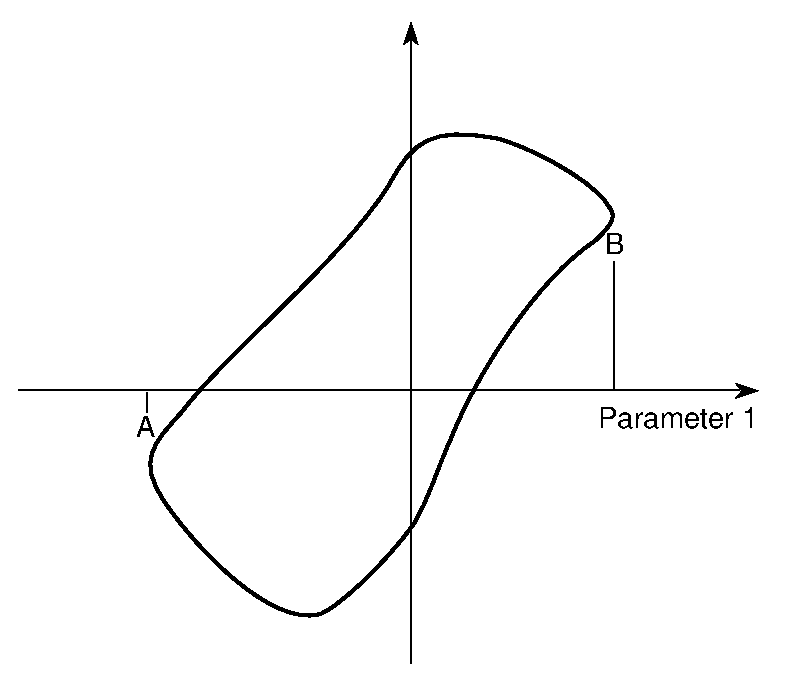
\includegraphics[width=\linewidth]{minoserr.eps}
\caption[MINOS errors for parameter 1]%
        {\Cind[MINos]{MINOS} errors for parameter 1}
\label{fig:MINoserror}
\end{minipage}\hfill
\begin{minipage}{.49\linewidth}
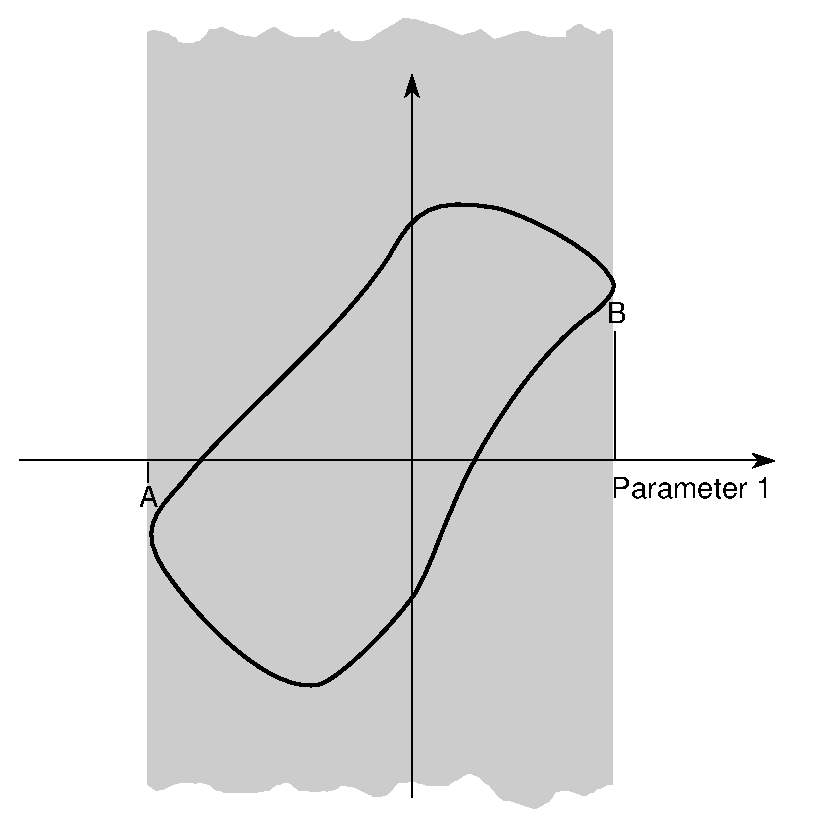
\includegraphics[width=\linewidth]{minosco1.eps}
\caption[MINOS error confidence region for parameter 1]%
        {\Cind[MINos]{MINOS} error confidence region for parameter 1}
\label{fig:MINosconf1}
\end{minipage}
\end{figure}
%end{latexonly}

\begin{htmlonly}
\begin{rawhtml}<P>\end{rawhtml}
\begin{figure}
\begin{makeimage}
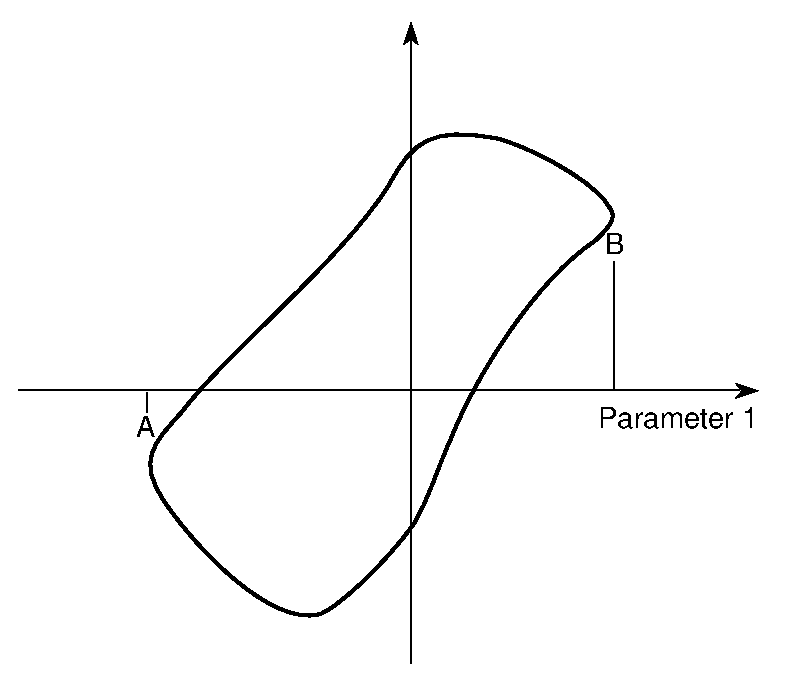
\includegraphics[width=\linewidth]{minoserr.eps}
\end{makeimage}
\caption{MINOS errors for parameter 1}
\label{fig:MINoserror}
\end{figure}

\begin{rawhtml}<P>\end{rawhtml}
\begin{figure}
\begin{makeimage}
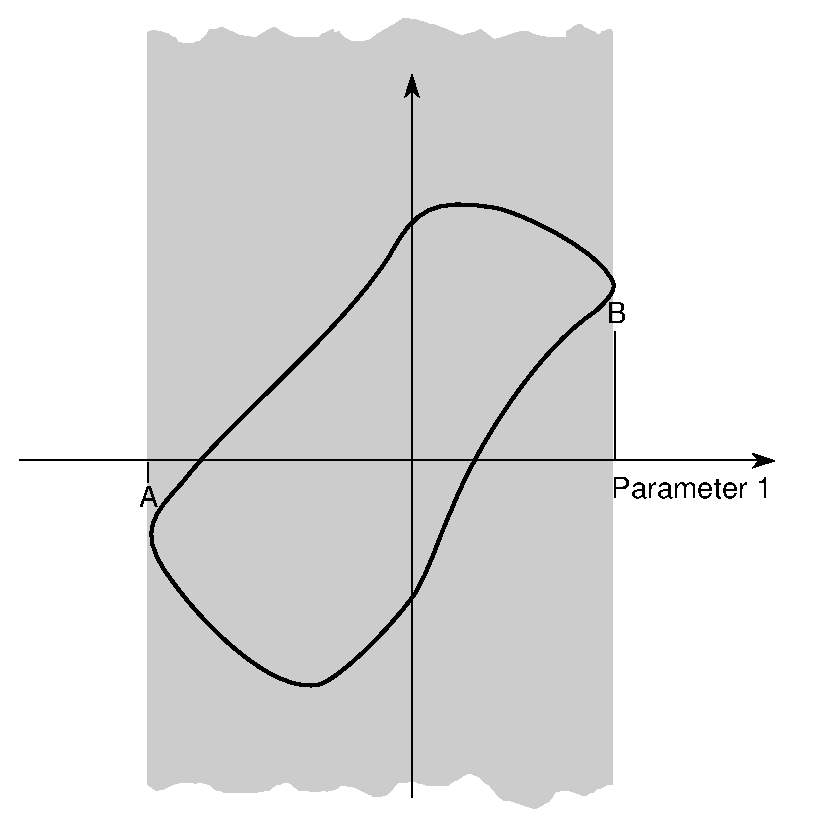
\includegraphics[width=\linewidth]{minosco1.eps}
\end{makeimage}
\caption{MINOS error confidence region for parameter 1}
\label{fig:MINosconf1}
\end{figure}
\begin{rawhtml}<P>\end{rawhtml}
\end{htmlonly}
 
If \texttt{UP} is set to the appropriate one-standard-deviation value, 
then the precise meaning of the confidence region of figure 
\ref{fig:MINosconf1} is:  ``The probability 
that the true value of parameter one lies between A and B is 68.3\%''
(the probability of a normally-distributed parameter lying within 
one std.-dev. of its mean). 
That is, the probability content of the 
grey area in figure \ref{fig:MINosconf1} is 68.3\%. 
No statement is made about 
the simultaneous values of the other parameter(s), since the grey
area covers all values of the other parameter(s).
 
If it is desired to make {\bf simultaneously} statements about the values 
of two or more parameters, the situation becomes considerably more 
complicated and the probabilities get much smaller. 
The first problem is 
that of choosing the shape of the confidence region, since it is no 
longer simply an interval on an axis, but a hypervolume. The easiest 
shape to express is the hyperrectangle given by: 

%begin{latexonly}
\begin{center}
\begin{tabular}{>{\tt}l}
A < param 1 < B \\
C < param 2 < D \\
E < param 3 < F , {\rm etc.}
\end{tabular}
\end{center}
%end{latexonly}
\begin{htmlonly}
\begin{alltt}
A < param 1 < B 
C < param 2 < D 
E < param 3 < F, \textrm{etc.}
\end{tabular}
\end{alltt}
\end{htmlonly}


This confidence region for our two-parameter example is the 
grey area in figure \ref{fig:MINosconf2}. 
However, there are two good reasons 
not to use such a shape:
 
\begin{enumerate}
\item Some regions inside the hyperrectangle (namely the corners) have 
      low likelihoods, lower than some regions just outside the rectangle, 
      so the hyperrectangle is not the optimal shape (does not contain the 
      most likely points).
\item One does not know an easy way to calculate the probability 
      content of these hyperrectangles (see~\cite{bib-EADIE}, p.196-197, 
      especially fig. 9.5a).
\end{enumerate} 

For these reasons one usually chooses regions delimited by contours 
of equal likelihood (hyperellipsoids in the linear case). For our 
two-parameter example, such a confidence region would be the grey
region in figure \ref{fig:MINosconf3}, and the corresponding probability 
statement is: ``The probability that parameter one and parameter two 
simultaneously take on values within the one-standard-deviation likelihood 
contour is 39.3\%''.
 
The probability content of confidence regions like those shaded in 
figure \ref{fig:MINosconf3} becomes very small as the number of parameters 
\texttt{NPAR} increases, for a given value of \texttt{UP}. 
Such probability contents are in 
fact the probabilities of exceeding the value \texttt{UP} for a chisquare 
function of \texttt{NPAR} degrees of freedom, and can therefore be read off 
from tables of chisquare. 
Table \ref{tab:MINosconf} gives the values of \texttt{UP} which 
yield hypercontours enclosing given probability contents for given 
number of parameters.

%begin{latexonly}
\begin{figure}[ht]
\begin{minipage}{.49\linewidth}
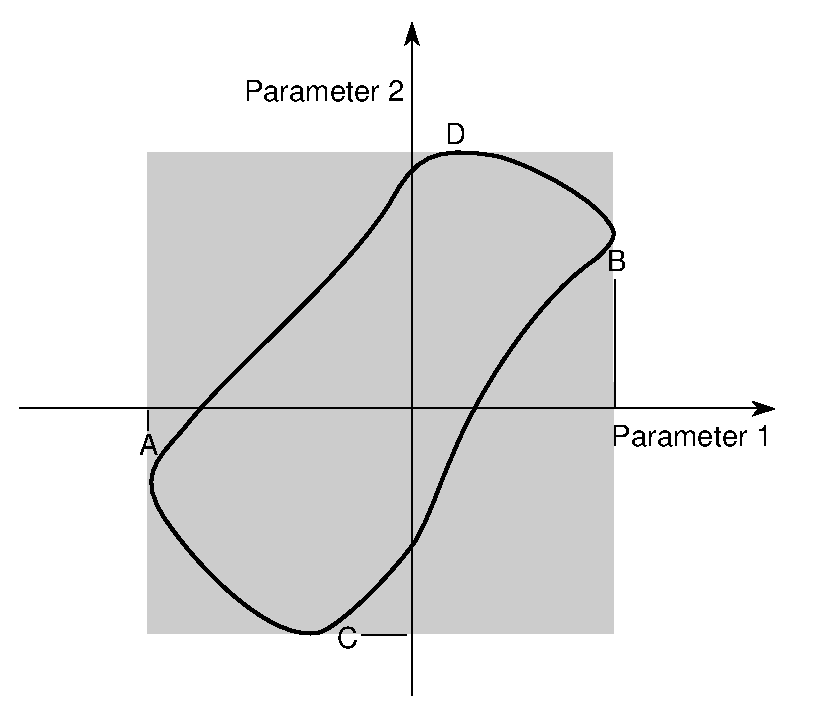
\includegraphics[width=\linewidth]{minosco2.eps}
\caption{Rectangular confidence region for parameters 1 and 2}
\label{fig:MINosconf2}
\end{minipage}\hfill
\begin{minipage}{.49\linewidth}
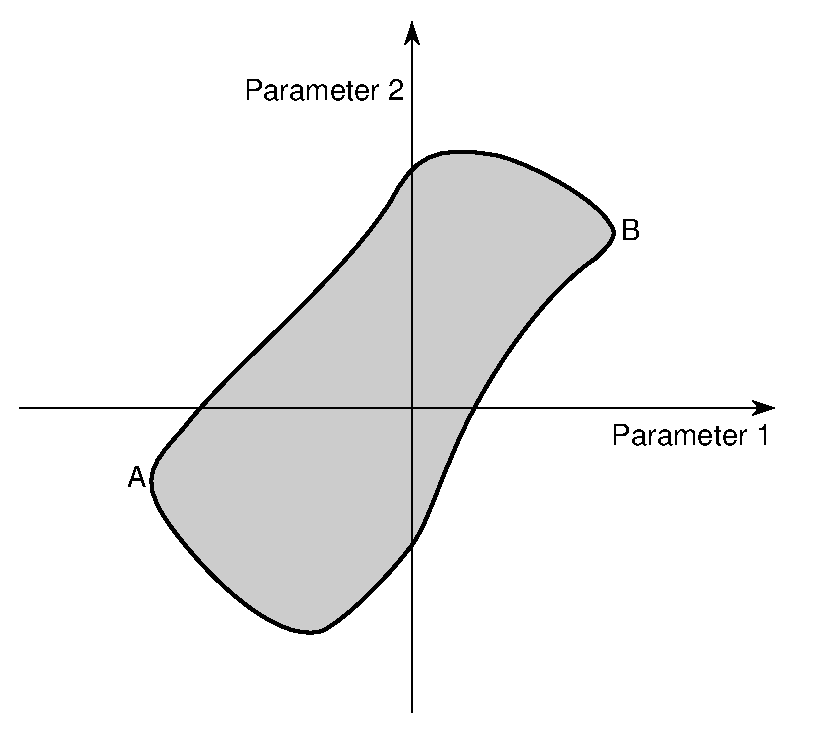
\includegraphics[width=\linewidth]{minosco3.eps}
\caption{Optimal confidence region for parameters 1 and 2}
\label{fig:MINosconf3}
\end{minipage}
\end{figure}
%end{latexonly}

\begin{htmlonly}
\begin{rawhtml}<P>\end{rawhtml}
\begin{figure}
\begin{makeimage}
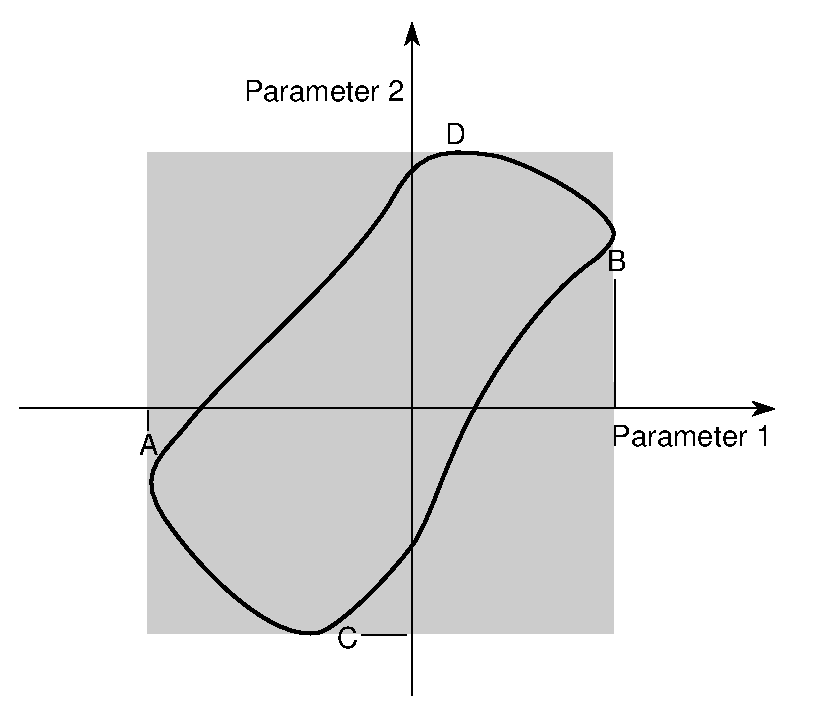
\includegraphics[width=\linewidth]{minosco2.eps}
\end{makeimage}
\caption{Rectangular confidence region for parameters 1 and 2}
\label{fig:MINosconf2}
\end{figure}

\begin{rawhtml}<P>\end{rawhtml}

\begin{figure}
\begin{makeimage}
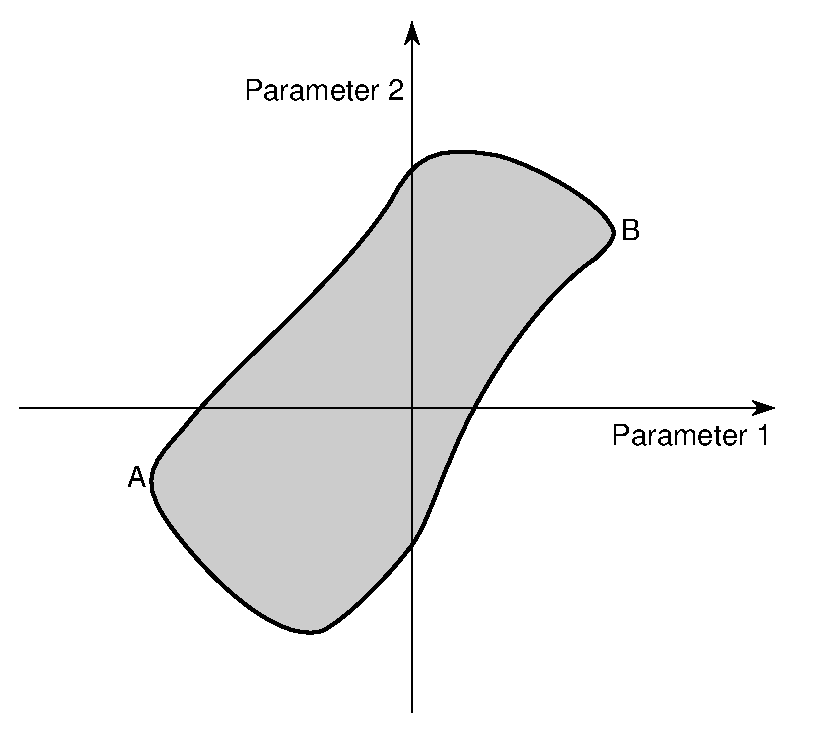
\includegraphics[width=\linewidth]{minosco3.eps}
\end{makeimage}
\caption{Optimal confidence region for parameters 1 and 2}
\label{fig:MINosconf3}
\end{figure}
\begin{rawhtml}<P>\end{rawhtml}
\end{htmlonly}
 
\begin{table}[th]
%begin{latexonly}
\begin{center}
\begin{tabular}{|r<{\quad}*{5}{|>{\quad}r<{\quad}}|} 
\hline
\multicolumn{1}{|r}{\ }
   & \multicolumn{5}{|l|}{\qquad Confidence level 
                              (probability contents desired inside}        \\
\multicolumn{1}{|r}{Number of} 
   & \multicolumn{5}{|l|}{\phantom{\qquad Confidence level (}hypercontour of 
                       $\chi^2 = \chi^2_{\mathrm{min}} + \mbox{\tt UP}$)}  \\
                       \cline{2-6}
\multicolumn{1}{|r|}{Parameters}
          & 50\%   &  70\%  &  90\%  &  95\%  &  99\%  \\
\hline 
1         &  0.46  &  1.07  &  2.70  &  3.84  &  6.63  \\
2         &  1.39  &  2.41  &  4.61  &  5.99  &  9.21  \\
3         &  2.37  &  3.67  &  6.25  &  7.82  & 11.36  \\
4         &  3.36  &  4.88  &  7.78  &  9.49  & 13.28  \\
5         &  4.35  &  6.06  &  9.24  & 11.07  & 15.09  \\
6         &  5.35  &  7.23  & 10.65  & 12.59  & 16.81  \\
7         &  6.35  &  8.38  & 12.02  & 14.07  & 18.49  \\
8         &  7.34  &  9.52  & 13.36  & 15.51  & 20.09  \\
9         &  8.34  & 10.66  & 14.68  & 16.92  & 21.67  \\
10        &  9.34  & 11.78  & 15.99  & 18.31  & 23.21  \\
11        & 10.34  & 12.88  & 17.29  & 19.68  & 24.71  \\
                       \cline{2-6}
& \multicolumn{5}{l|}{\qquad If \protect\Rind{FCN} is $-\log(\mathrm{likelihood})$
                             instead of $\chi^2$, all values of \texttt{UP} }        \\
& \multicolumn{5}{l|}{\qquad should be divided by 2.}                             \\
\hline
\end{tabular}
\end{center}
%end{latexonly}
\begin{htmlonly}
\begin{tabular}{|r|r|r|r|r|r|}
   & \multicolumn{5}{|c|}{Confidence level}\\
\multicolumn{1}{|r}{Nb. parameters}
   & \multicolumn{5}{|c|}{(probability contents desired inside hypercontour
                       $\chi^2 = \chi^2_{\mathrm{min}} + \mathtt{UP}$)}  \\
          & 50\%   &  70\%  &  90\%  &  95\%  &  99\%  \\
1         &  0.46  &  1.07  &  2.70  &  3.84  &  6.63  \\
2         &  1.39  &  2.41  &  4.61  &  5.99  &  9.21  \\
3         &  2.37  &  3.67  &  6.25  &  7.82  & 11.36  \\
4         &  3.36  &  4.88  &  7.78  &  9.49  & 13.28  \\
5         &  4.35  &  6.06  &  9.24  & 11.07  & 15.09  \\
6         &  5.35  &  7.23  & 10.65  & 12.59  & 16.81  \\
7         &  6.35  &  8.38  & 12.02  & 14.07  & 18.49  \\
8         &  7.34  &  9.52  & 13.36  & 15.51  & 20.09  \\
9         &  8.34  & 10.66  & 14.68  & 16.92  & 21.67  \\
10        &  9.34  & 11.78  & 15.99  & 18.31  & 23.21  \\
11        & 10.34  & 12.88  & 17.29  & 19.68  & 24.71  \\
                       \cline{2-6}
& \multicolumn{5}{l|}{For \protect\Rind{FCN} $-\log(\mathrm{likelihood})$
                      instead of $\chi^2$, all values of
                      \texttt{UP} to be divided by 2.}                             
\end{tabular}
\end{htmlonly}
\caption{Table of \texttt{UP} for multi-parameter confidence regions}
\label{tab:MINosconf}
\end{table}

 
